\documentclass[a4paper,12pt]{article}

\usepackage{../usfdvl}

\title{Project 0: Introduction to Processing}
\SetDocumentFooter{}{}


\begin{document}

\maketitle

\projectGroundRules

\projectSubmission


\vspace{5pt}
\section{Assignment Instructions}

\vspace{5pt}
\myparagraph{This assignment will help you become familiar with Processing and build some basic data structures for storing geometric data.}

\begin{itemize}

\item Download and familiarize yourself with Processing (\url{http://processing.org/download/}). Use the available tutorials (\url{http://processing.org/tutorials/}) and examples (\url{http://processing.org/examples/}) to help you understand how Processing works.
 

\item Use the provided skeleton code, first fill in all of the \texttt{TODO} items.
\item Then complete a sketch with the following requirements.

\begin{minipage}[b]{0.58\textwidth}
\begin{itemize}

\item When the mouse is clicked, a new point should be added to the point list. This point should be drawn using an ellipse and include a label.

\item Every point should be connected to the previously added point with an edge in the edge list. The edges list should be drawn every frame. When the edge is created, the edge's \texttt{printInfo()} function should be called to display information about the new edge.

\item Every 3 points should form a triangle that is added to the triangle list. The triangles should be drawn and colored based upon whether they are stored in a clockwise or counterclockwise order. When the triangle is created, the triangle's \texttt{printInfo()} function should be called to display information about the new triangle.

\end{itemize}
\end{minipage}
%
\hfill
%
\begin{minipage}[b]{0.325\textwidth}
\begin{center}
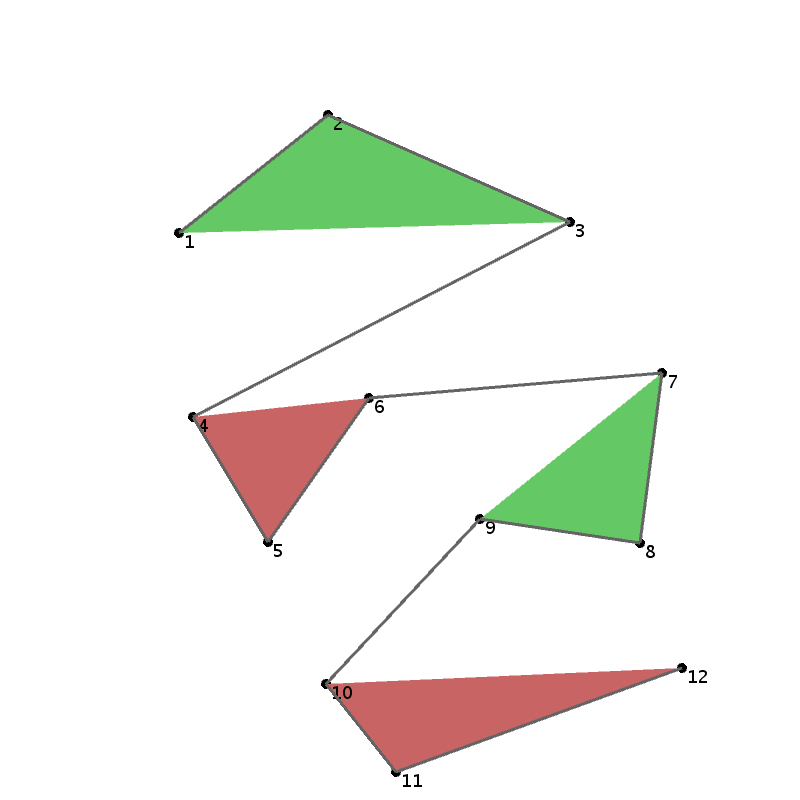
\includegraphics[width=0.975\linewidth]{../images/project0.png}
Example output.
\end{center}
\end{minipage}


\end{itemize}






\end{document}
